\documentclass{article}
\usepackage[polish]{babel}
\usepackage[utf8]{inputenc}
\usepackage{polski}
\usepackage{hyperref}
\frenchspacing
\setcounter{tocdepth}{2}
\usepackage{graphicx}
\graphicspath{ {images/} }
\usepackage{float}

\begin{document}
	
\begin{titlepage}

\newcommand{\HRule}{\rule{\linewidth}{0.5mm}}

\center

%----------------------------------------------------------------------------------------

\textsc{\LARGE Politechnika Warszawska}\\[10mm]
\textsc{\LARGE Wydział Matematyki i Nauk}\\[4mm]
\textsc{\LARGE Informacyjnych}\\[4cm]
 
%----------------------------------------------------------------------------------------

\textsc{\Huge Metody Data Science}\\[0.5cm]

%----------------------------------------------------------------------------------------

\HRule \\[0.4cm]
{ \LARGE \bfseries Moduł pozyskiwania danych}\\[5.0cm]
 
 
%----------------------------------------------------------------------------------------

\begin{flushright}
\Large \emph{Autorzy:}\\[0.5cm]
Piotr \textsc{Izert}\\
Przemysław \textsc{Rząd}\\
Anna \textsc{Zawadzka}\\
\end{flushright}

%----------------------------------------------------------------------------------------

\vfill
{\large \today}\\[3cm]

\end{titlepage}
	
\newpage

\section{Wstęp}

Niniejszy projekt ma na celu wykonanie uczącego się systemu, który na podstawie pobieranych danych po odpowiednim ich przetworzeniu przygotowuje analizę w postaci prognozowania oraz  klasyfikacji.\\

Projekt polega na zebraniu oraz odpowiednim przetworzeniu danych zawierających informacje o wypadkach drogowych na terenie Wielkiej Brytanii, uczestniczących w nich pojazdach oraz poszkodowanych. Używane będą także informacje o prędkościach przejazdu samochodów na określonych odcinkach dróg. \\

Wynikiem przetworzenia danych będą prognozy o możliwych wypadkach w zależności od różnych czynników oraz lokalizacji, a także klasyfikacja na bieżąco napływających danych o wypadkach ze względu na ich skalę.\\

Dzięki takiej analizie i prognozowaniu możliwe będzie skoordynowanie rozmieszczenia  patroli policji zgodnie z przewidywaniami, a także dzięki klasyfikacji wypadków na poważne i mniej groźne, wiadomo będzie, do którego zdarzenia należy wysłać więcej karetek pogotowia, bądź innych służb porządkowych, co może znacznie usprawnić reagowanie na takie zdarzenia.

%----------------------------------------------------------------------------------------

\section{Dane}

Źródłem danych są zbiory udostepnione przez ministerstwo transportu rządu Wielkiej Brytanii na stronach internetowych:
\begin{itemize}
    \item \url{https://data.gov.uk/dataset/road-accidents-safety-data}
    \item \url{https://data.gov.uk/dataset/dft-eng-srn-routes-journey-times}
\end{itemize}
Dane obejmują informacje na temat wypadków drogowych na terenie Wielkiej Brytanii oraz średnich prędkościach przejazdu samochodów na danych odcinkach dróg w latach 2009-2014. Przechowywane są w plikach o formacie CSV. Dane pobierane są jako zamknięty zbiór rekordów, natomiast wykorzystane będą jako dane napływające w czasie rzeczywistym. \\\\
Dane na temat wypadków zawierają 4 kategorie plików:
\begin{itemize}
    \item Wypadki
    \item Poszkodowani
    \item Pojazdy
    \item Marki pojazdów
\end{itemize}
Poniższa tabela prezentuje liczbę zmiennych (wszystkich, niezależnych i zależnych) w plikach z poszczególnych kategorii:\\

\begin{tabular}{|r|r|r|r|r|}
  \hline 
    & Wypadki & Pojazdy & Poszkodowani & Marki pojazdów\\
  \hline 
  Wszystkie & 32 & 21 & 14 & 24\\
  \hline
  Niezależne & 27 & 21 & 14 & 23\\
  \hline
  Zależne & 5 & 0 & 0 & 1\\
  \hline
\end{tabular} \\[0.5cm]
Pliki z danymi o wypadkach zawierają następujące zmienne zależne: %TODO: opisac po polsku
\begin{itemize}
    \item  Dzień tygodnia
    \item  Długość geograficzna w formacie OSGR 
    \item  Szerokość geograficzna w formacie OSGR 
    \item  Dystrykt
    \item  Władze lokalne w formacie kodu ONS
\end{itemize}\\
Dane zawierające informacje o pojazdach wraz z markami i modelami zawierają 9 zmiennych, w tym jedną zmienną zależną - rok, w którym doszło do wypadku z udziałem danego pojazdu. Informację tę można uzyskać bezpośrednio z indentyfikatora wypadku.\\\\
Poniższa tabela reprezentuje liczbę rekordów w plikach danych kategorii w każdym roku:\\

\begin{tabular}{|r|r|r|r|r|}
  \hline 
    & Wypadki & Pojazdy & Poszkodowani & Marki pojazdów\\
  \hline 
  2009 & 163555 & 298688 & 222147 & 182322\\
  \hline
  2010 & 154415 & 281402 & 208649 & 180368\\
  \hline
  2011 & 151475 & 276156 & 203951 & 180617\\
  \hline
  2012 & 145572 & 265878 & 195724 & 173860\\
  \hline
  2013 & 138661 & 252914 & 183671 & 171626\\
  \hline
  2014 & 146323 & 268528 & 194478 & 182354\\
  \hline
\end{tabular} \\[0.3cm]
Łączny rozmiar tych danych (po 4 pliki dla każdego roku) to 377 MB.\\\\
Dane zawierające informacje o prędkościach przejazdu na określonych odcinkach dróg podzielone są ze względu na rok i miesiąc, łącznie 72 pliki CSV. Średnio rozmiar każdego pliku to 0.8 GB, zatem rozmiar całego zestawu danych zawierających informacje o prędkościach przejazdów to 57.6 GB.\\
Dane te zawierają jędną zmienną zależną, jest to opis odcinka drogi (wskazanie skrzyżowań, między którymi znajduje się określony odcinek drogi).\\\\
W projekcie używane będą również tabele słownikowe, których rozmiar to 447 KB. Będą one wczytywane jednorazowo i nie będą podlegać zmianie w trakcie działania systemu.

%----------------------------------------------------------------------------------------

\section{Moduł pozyskiwania danych}

Użyte narzędzia:
\begin{itemize}
    \item maszyna wirtualna Hortonworks Sandbox (HDP 2.4)
    \item Flume
    \item Spark
    \item HDFS
\end{itemize}

\begin{figure}[H]
\centering
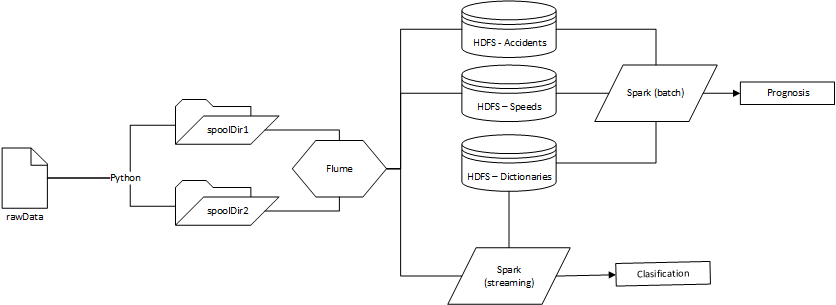
\includegraphics[scale=0.6]{schemat}
\caption{Schemat modułu pozyskiwania danych}
\end{figure}

W katalogu \textit{rawData} na maszynie wirtualnej umieszczone zostaną pliki w formacie CSV pięciu kategorii: wypadki, samochody, marki i modele samochodów, ofiary oraz średnie prędkości na poszczególnych odcinkach dróg. Dane o wypadkach, ofiarach, samochodach oraz ich markach i modelach pogrupowane są w pliki ze względu na rok, natomiast dla danych o prędkościach istnieją osobne pliki dla każdego miesiąca w danym roku.

Następnie za pomocą skryptu napisanego w języku Python zostaną połączone pliki z danymi o wypadkach, ofiarach, samochodach oraz ich markach i modelach dla każdego roku (za pomocą instrukcji SQL). Pliki wynikowe (osobne dla każdego roku) będą zawierać dane o wypadkach, samochodach w nich uczestniczących wraz z informacją o markach i modelach oraz ofiarach tychże wypadków.

Do każdego wypadku przyporządkowanych jest zawsze kilka samochodów, natomiast nie dla wszystkich pojazdów istnieje informacja o ofiarach (poszkodowani przyporządkowani są do konkretnego pojazdu) oraz o marce i modelu.

Nowo utworzone pliki zostaną automatycznie skopiowane do katalogu \textit{spoolDir1} (\textit{spooling directory}), który jest specjalnym katalogiem monitorowanym przez Flume’a. Dane o prędkościach przejazdów będą automatycznie umieszczane w katalogu \textit{spoolDir2} bez żadnych zmian. Jeżeli w katalogach \textit{spooling} pojawiają się w nim nowe pliki, Flume rozpoczyna ich przetwarzanie.

Konfiguracja Flume’a zakłada istnienie dwóch źródeł (\textit{source}), którymi są \textit{spoolDir1} i \textit{spoolDir2}, oraz czterech ujść (\textit{sink}), po dwa dla HDFS’a i dla Spark’a, odpowiednio dla skonsolidowanych danych o wypadkach oraz dla danych o prędkościach przejazdów. Ujścia skierowane do HDFS’a odwoływać się będą do katalogów \textit{Accidents} oraz \textit{Speeds}, natomiast ujścia do Spark’a odwołują się do odpowiedniego Job’a, który przetworzy dane w sposób strumieniowy.

W systemie HDFS istnieje dodatkowo katalog \textit{Dictionaries}, w którym umieszczone są pliki słownikowe, wykorzystywane w dalszych etapach projektu. Pliki w tym katalogu umieszczone będą ręcznie i jednorazowo.  

Dane ze wszystkich katalogów w HDFS (\textit{Accidents}, \textit{Speeds}, \textit{Dictionaries}) pobierane będą przez Job’a (Spark) w sposób wsadowy i używane do generowania prognoz.

Przetwarzanie strumieniowe także korzystać będzie z danych znajdujących się w HDFS w katalogu Dictionaries i będzie realizować zadanie klasyfikacji.


\section{Zadania modułu analitycznego}

Moduł analityczny zostanie zrealizowany za pomocą oprogramowania Spark i będzie korzystał z danych przygotowanych przez moduł pozyskiwania danych. Zadaniem modułu analitycznego będzie:
\begin{itemize}
    \item generowanie okresowych prognoz liczby wypadków w danym rejonie
    \item przewidywanie w trybie \emph{on-line} liczby ofiar i rodzaju ich obrażeń na podstawie danych o zdarzeniu drogowym
\end{itemize}

W celu generacji okresowych prognoz, dane będą przetwarzane w trybie wsadowym. Do generacji prognozy np. na konkretny tydzień zostaną użyte dane z całego wcześniejszego okresu od początku dostępności danych.

Odpowiadanie na pytanie o stopień obrażeń uczestników wypadku zrealizowane zostanie przez przetwarzanie napływających danych w symulowanym trybie strumieniowym. System będzie miał do dyspozycji informacje o analizowanym zdarzeniu drogowym z wyjątkiem liczby ofiar i ich obrażeń oraz pełną informacje o wcześniej przetworzonych zdarzeniach.

\end{document}



